\documentclass[12pt,a4paper,oneside]{report}

%==================== PACKAGES ====================
\usepackage[utf8]{inputenc}
\usepackage[T1]{fontenc}
\usepackage[french]{babel}
\usepackage{lmodern}
\usepackage{geometry}
\geometry{top=2.5cm,bottom=2.5cm,left=3cm,right=2.5cm}
\usepackage{setspace}
\onehalfspacing
\usepackage{graphicx}
\usepackage{float}
\usepackage{booktabs}
\usepackage{array}
\usepackage{titlesec}
\usepackage{fancyhdr}
\usepackage{tocloft}
\usepackage{hyperref}
\usepackage{xcolor}

%==================== STYLE ====================
\definecolor{main}{RGB}{0,60,120}

\titleformat{\chapter}[display]
{\bfseries\Huge\color{main}}
{\filleft\Huge\chaptername\ \thechapter}
{1ex}
{\titlerule\vspace{1ex}\filright}

\pagestyle{fancy}
\fancyhf{}
\fancyhead[L]{Rapport de stage}
\fancyhead[R]{\thepage}

%==================== DOCUMENT ====================
\begin{document}

%==================== PAGE DE GARDE ====================
% \begin{titlepage}
% \centering

% {\Large RÉPUBLIQUE ALGÉRIENNE DÉMOCRATIQUE ET POPULAIRE}\\[0.5cm]
% {\large MINISTÈRE DE LA DÉFENSE NATIONALE}\\[0.3cm]
% {\large ÉCOLE MILITAIRE POLYTECHNIQUE}\\[2cm]
% \begin{figure}[h!]
% \centering

% \begin{minipage}{0.45\textwidth}
%     \centering
%     
\includegraphics[width=\linewidth]{./images/unita.png}
% \end{minipage}
% \hfill
% \begin{minipage}{0.45\textwidth}
%     \centering
%     
\includegraphics[width=\linewidth]{./images/ecrmt.png}
% \end{minipage}

% \end{figure}

% {\Huge \textbf{Rapport de stage}}~\\

% {\Large ~\\ Conception d'un circuit  mouvement sinusoïdale d'une MCC
% ~\\
% }~\\

% \begin{flushleft}

% \textbf{Réalisé par :}\\
% EOC. Bouziane Touka Hibat Allah\\
% EOC. Boudouha Jihane \\[1cm]

% \textbf{Encadré par :}\\
% Cne. BOUAHMED Ayoub Imed Eddine \\

% \end{flushleft}

% \vfill

% {\large Année Universitaire 2025--2026}

% \end{titlepage}

%==================== REMERCIEMENTS ====================
\chapter*{Remerciements}
\addcontentsline{toc}{chapter}{Remerciements}

Nous tenons tout d’abord à remercier Allah le tout-puissant et miséricordieux, qui nous a donné la force, la patience, la volonté et le courage pour la réussite dans nos études. En second lieu, nous tenons à témoigner nos vifs remerciements à nos encadreur le capitane «BOUAHMED Ayoub Imed Eddine» et madame «Tekamera Dalila » pour leur précieux conseils et leur aide durant toute la période du travail, et tous les officiers du laboratoire central de recherche et développement
pour leurs conseils judicieux, leur aide et leur disponibilité. Nos vifs remerciements vont également aux membres du jury pour l’intérêt qu’ils ont porté à notre travail en acceptant de l’examiner et de l’enrichir par leurs propositions. Enfin, nous tenons également à remercier toutes les personnes qui ont participé de près ou de loin à la réalisation de ce travail.

%==================== TABLE ====================




% ================= INTRODUCTION =================



\chapter*{Introduction générale}
\addcontentsline{toc}{chapter}{Introduction générale}

Dans le cadre de ce stage, un système de génération de mouvement sinusoïdal pour le contrôle  d'une machine à courant continu a été étudié et réalisé. Ce système repose principalement sur la génération d’un signal PWM (Pulse Width Modulation), utilisé comme base de commande.

Dans un premier temps, un signal PWM est généré afin de représenter l’évolution souhaitée de la tension appliquée au moteur. Ce type de signal permet de contrôler efficacement la puissance fournie tout en garantissant une bonne précision de commande.

Par la suite, afin d’assurer l’inversion du sens de rotation du moteur, un pont en H est utilisé. Ce circuit électronique permet la commutation de la polarité appliquée au moteur, et joue un rôle essentiel dans le contrôle du sens de rotation.

Le pont en H est  Contrôlé par un signal PWM et son signal complémentaire., ce qui permet d’assurer une inversion contrôlée du tension et une transition fluide du mouvement.



\chapter{Présentation de l'unité d'accueil}
\label{chap:presentation_unite}

\section{Introduction}
\label{sec:intro_ch1}

L’Établissement Central de Rénovation du Matériel des Transmissions/1°RM (ECRMT), en tant qu’organe principal de la chaîne de soutien de l’Arme des Transmissions et des Systèmes d’Information, assure l’ensemble des missions assignées en termes de maintien en condition des moyens des transmissions en déploiement au sein des différentes structures de l’ANP. Dans ce chapitre, nous allons décrire l’organisation, les missions et les processus de production de l’établissement, avec un focus particulier sur le Département d’Assemblage des Moyens de Commutation et le Laboratoire Central de Recherche et Développement.

\section{Missions de l'ECRMT}
\label{sec:missions_ecrmt}

L’établissement est l’organe central du soutien technique des Transmissions au profit des forces, des unités et des structures du Ministère de la Défense Nationale. Il est chargé principalement des missions suivantes :

\paragraph{En termes de production}
\begin{itemize}
    \item L’assemblage des équipements, des parties d’équipements, sous-ensembles et accessoires des transmissions ou entrant dans la composition des équipements des transmissions et de guerre électronique.
\end{itemize}

\paragraph{Maintenance, Rénovation et Installation}
\begin{itemize}
    \item Rénovation des équipements de transmissions ;
    \item Maintenance du matériel des transmissions échelon 3° et 4° ;
    \item Le contrôle et l’évaluation techniques des moyens réalisés par la Direction Centrale des Transmissions et des Systèmes d’Information (DCTSI) ;
    \item La maintenance, l’administration et la supervision des réseaux de transmissions ;
    \item L’étude de faisabilité et l’installation des équipements de transmissions sur site et à bord des engins tactiques.
\end{itemize}

\paragraph{Développement, Formation et Veille technologique}
\begin{itemize}
    \item La formation spécialisée du personnel technicien sur les équipements de transmissions nouvellement acquis et l’organisation de stages pratiques ;
    \item L’établissement met au profit de la Direction Centrale des Transmissions des rapports de synthèse, d’analyse et de veille technologique ;
    \item L’établissement des audits internes des activités d’assemblage et de rénovation ;
    \item Assurer les coopérations, en termes de diffusion et de capitalisation des connaissances techniques, avec les différentes structures de Recherches et Développement.
\end{itemize}

\section{Structure Organisationnelle de l'ECRMT}
\label{sec:structure_ecrmt}

\begin{figure}[H]
    \centering
    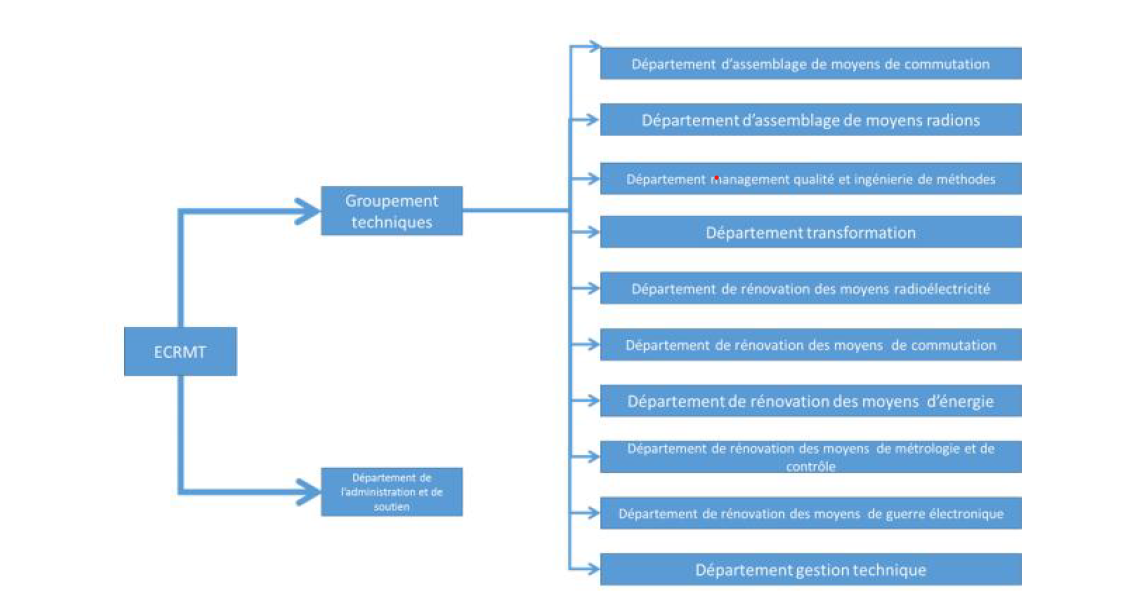
\includegraphics[width=0.9\textwidth]{./images/organigramme_ecrmt.png}
    \caption{Organigramme de la structure organisationnelle de l’ECRMT.}
    \label{fig:organigramme_ecrmt}
\end{figure}

\subsection{Département d'Assemblage des Moyens de Commutation}
\label{subsec:dept_assemblage}

Le Département d’Assemblage des Moyens de Commutation a pour mission la production des moyens de commutation. Son objectif stratégique est de gérer à terme la chaîne de montage de manière autonome, sans assistance étrangère, afin de maîtriser la production complète de tout équipement de transmissions.

\subsection{Processus d'assemblage}
\label{subsec:processus_assemblage}

Les processus d’assemblage sont organisés par zones, suivant le flux de production depuis la réception des composants jusqu’à la livraison du produit fini.

\paragraph{Magasin (Warehouse)}

\begin{figure}[H]
    \centering
     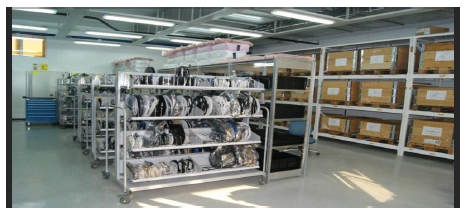
\includegraphics[width=0.8\textwidth]{./images/magasin.png}
    \caption{Vue du magasin (Warehouse) de l'ECRMT}
    \label{fig:magasin}
\end{figure}

Le processus d'assemblage débute au niveau du magasin par les étapes suivantes :
\begin{itemize}
    \item Réception et vérification des composants et consommables ;
    \item Enregistrement sur la base de données du système ERP ;
    \item Saisie des données de traçabilité (référence, date de fabrication, fabricant, etc.) pour chaque lot ;
    \item Préparation des kits de composants selon le plan de production.
\end{itemize}

\begin{figure}[H]
    \centering
     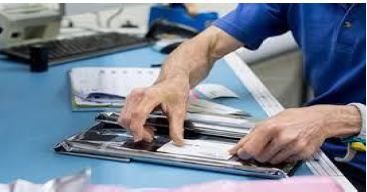
\includegraphics[width=0.8\textwidth]{./images/erp_interface.png}
    \caption{Interface du système de Gestion ERP utilisé à l'ECRMT}
    \label{fig:erp_interface}
\end{figure}

\textbf{Note :} La chaîne d'assemblage des moyens radio dispose d'un système de stockage automatisé avec 10 500 emplacements pour composants.

\begin{figure}[H]
    \centering
     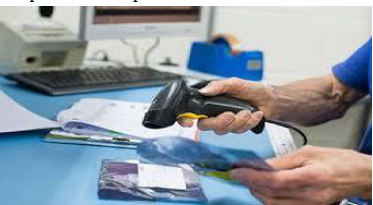
\includegraphics[width=0.8\textwidth]{./images/stockage_auto.png}
    \caption{Système de stockage automatisé de la chaîne d'assemblage des moyens radio}
    \label{fig:stockage_auto}
\end{figure}

\paragraph{Zone de production}

Cette zone comprend les lignes d'assemblage des cartes électroniques et les lignes d'assemblage final des produits.

\subsection{Lignes d'assemblage des cartes électroniques}
\label{subsec:lignes_electroniques}

Cette partie universelle de la chaîne d'assemblage se divise en deux types de lignes selon les composants utilisés.

\subsubsection*{Ligne d'assemblage SMT}

Dédiée à l'assemblage automatique des cartes électroniques à base de composants montés en surface (Surface Mount Technology).

\begin{figure}[H]
    \centering
    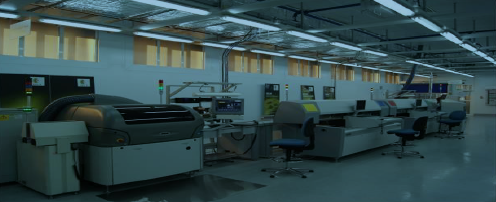
\includegraphics[width=0.8\textwidth]{./images/ligne_smt.png}
    \caption{Vue générale de la ligne d'assemblage SMT}
    \label{fig:ligne_smt}
\end{figure}

\textbf{Processus de la ligne SMT}

\begin{enumerate}
    \item \textbf{Sérigraphie :} Étendage automatique de la pâte à braser sur les circuits imprimés à l’aide de pochoirs (stencils) spécifiques.
    
    \begin{figure}[H]
        \centering
         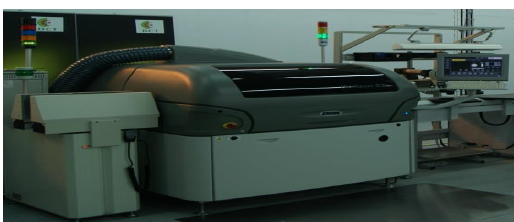
\includegraphics[width=0.6\textwidth]{./images/serigraphie.png}
        \caption{Machine de sérigraphie pour l’application de la pâte à braser}
        \label{fig:serigraphie}
    \end{figure}
    
    Ce processus est critique car il représente 60 à 70\% des erreurs de production.
    
    \item \textbf{Placement automatique des composants :} Positionnement précis des composants sur le circuit imprimé.
    
    \begin{figure}[H]
        \centering
         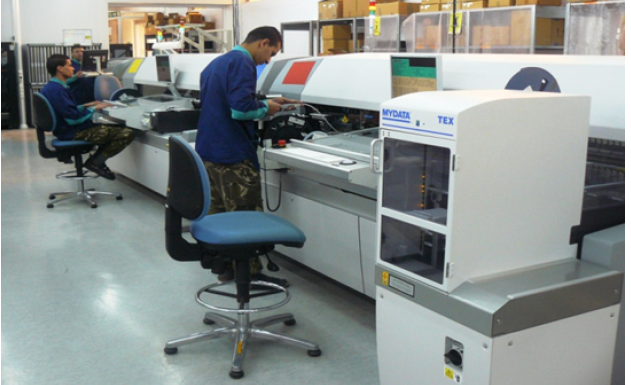
\includegraphics[width=0.6\textwidth]{./images/pick_and_place.png}
        \caption{Machine de placement automatique des composants (Pick \& Place)}
        \label{fig:pick_place}
    \end{figure}
    
    \textbf{Capacités des machines de placement :}
    \begin{itemize}
        \item Chaîne d'Assemblage des Moyens Radio : 90 000 composants/heure (3 machines $\times$ 30 000/heure)
        \item Chaîne d'Assemblage des Moyens de Commutation : 64 000 composants/heure (2 machines $\times$ 32 000/heure)
    \end{itemize}
    
    \item \textbf{Soudure par refusion :} Passage des cartes dans un four à refusion avec profils de température préprogrammés.
    
    \item \textbf{Inspection Optique Automatique (AOI) :} Vérification automatique de la présence, orientation et qualité des soudures.
    
    \item \textbf{Inspection par rayons X :} Contrôle des composants non visibles optiquement.
    
    \item \textbf{Inspection visuelle :} Contrôle complémentaire après sérigraphie et placement.
\end{enumerate}

\subsubsection*{Ligne d'assemblage THT}

Dédiée à l’assemblage manuel et semi-automatique des cartes à composants traversants (Through-Hole Technology).

\begin{figure}[H]
    \centering
     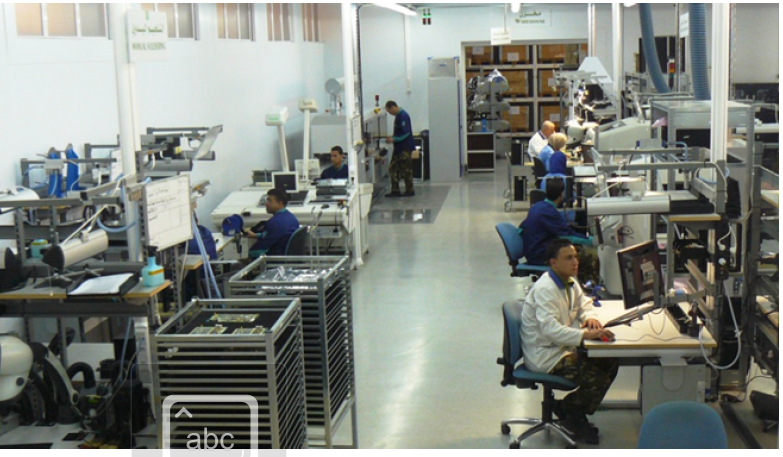
\includegraphics[width=0.8\textwidth]{./images/ligne_tht.png}
    \caption{Vue générale de la ligne d’assemblage THT}
    \label{fig:ligne_tht}
\end{figure}

\textbf{Processus de la ligne THT}

\begin{enumerate}
    \item \textbf{Préparation des composants (préformage) :} Coupe et mise en forme des pattes des composants.
    
    \item \textbf{Placement des composants :} Insertion manuelle ou semi-automatique des composants traversants.
    
    \begin{figure}[H]
        \centering
        \begin{minipage}{0.48\textwidth}
            \centering
             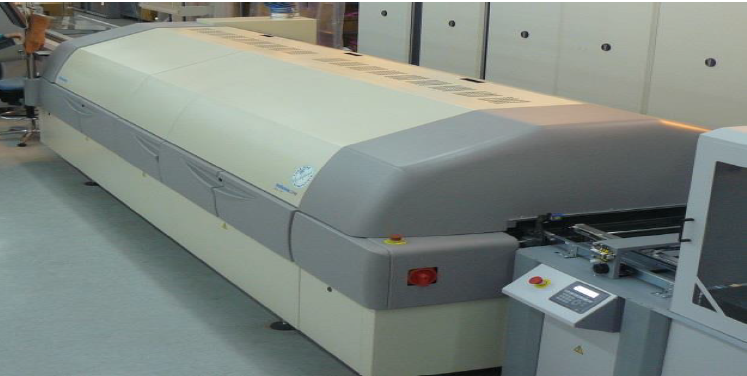
\includegraphics[width=\textwidth]{./images/placement_semi_auto.png}
            \caption{Placement semi-automatique des composants THT}
            \label{fig:placement_semi_auto}
        \end{minipage}\hfill
        \begin{minipage}{0.48\textwidth}
            \centering
            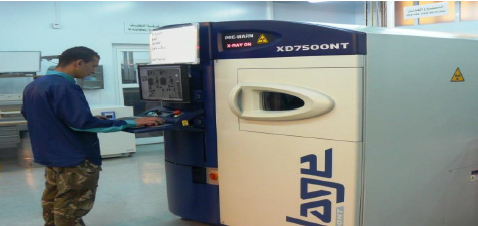
\includegraphics[width=\textwidth]{./images/placement_manuel.png}
            \caption{Placement manuel des composants THT}
            \label{fig:placement_manuel}
        \end{minipage}
    \end{figure}
    
    \item \textbf{Soudure des composants :} Réalisée par soudure sélective robotisée, soudure à la vague ou manuelle.
    
    \begin{figure}[H]
        \centering
         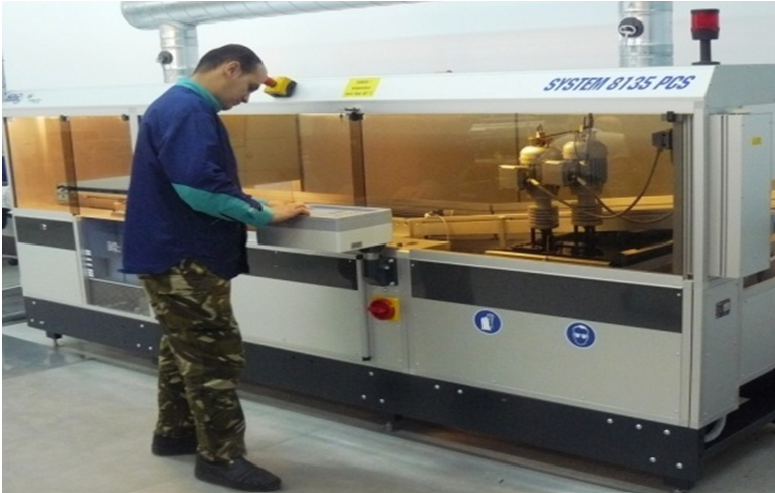
\includegraphics[width=0.7\textwidth]{./images/soudure_tht.png}
        \caption{Processus de soudure des composants THT}
        \label{fig:soudure_tht}
    \end{figure}

    \item \textbf{Inspection visuelle :} Contrôle qualité des joints de soudure.
    
    \begin{figure}[H]
        \centering
         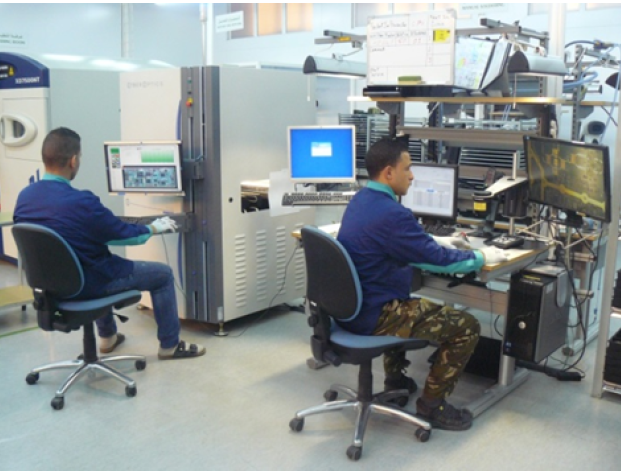
\includegraphics[width=0.8\textwidth]{./images/inspection_visuelle_tht.png}
        \caption{Exemples d'inspection visuelle des soudures THT}
        \label{fig:inspection_visuelle_tht}
    \end{figure}

    \item \textbf{Nettoyage des cartes :} Élimination des résidus chimiques (disponible sur la chaîne de commutation).
    
    \begin{figure}[H]
        \centering
         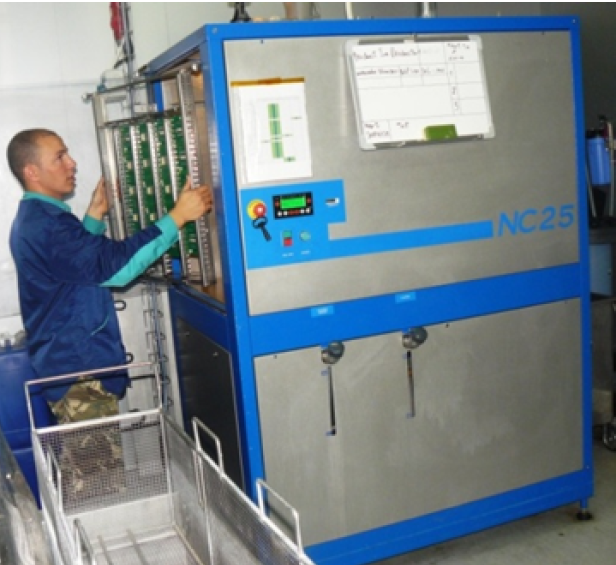
\includegraphics[width=0.6\textwidth]{./images/nettoyage_cartes.png}
        \caption{Station de nettoyage des cartes électroniques}
        \label{fig:nettoyage_cartes}
    \end{figure}
    
    Utilisation d'un mélange eau déminéralisée/alcool spécialisé.

    \item \textbf{Test des cartes :} Tests électriques, fonctionnels et chargement des logiciels.
    
    \begin{figure}[H]
        \centering
         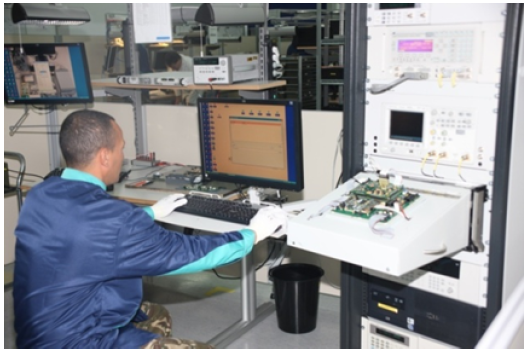
\includegraphics[width=0.6\textwidth]{./images/test_cartes.png}
        \caption{Station de test automatisé des cartes électroniques}
        \label{fig:test_cartes}
    \end{figure}
\end{enumerate}

\subsection{Lignes d'assemblage final}
\label{subsec:lignes_final}

\paragraph{Assemblage final}

Assemblage des différents sous-ensembles pour former les produits finis.

\begin{figure}[H]
    \centering
     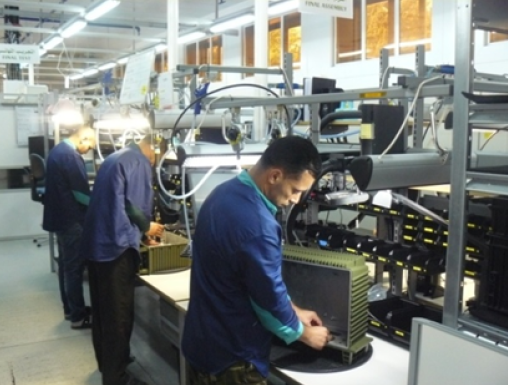
\includegraphics[width=0.8\textwidth]{./images/assemblage_final.png}
    \caption{Ligne d'assemblage final des produits}
    \label{fig:assemblage_final}
\end{figure}

\paragraph{Test final}

Tests conformes à la norme militaire MIL-STD-810 : fonctionnels, étanchéité, température, vibration.

\begin{figure}[H]
    \centering
    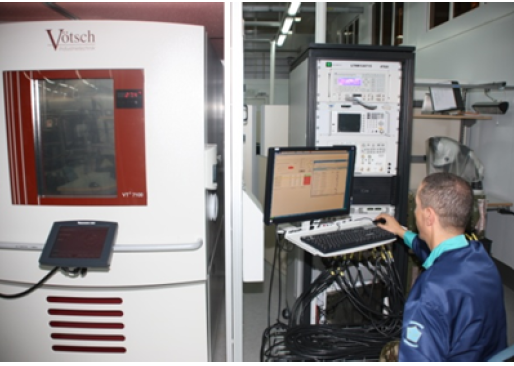
\includegraphics[width=0.8\textwidth]{./images/chambre_environnementale.png}
    \caption{Chambre de test environnemental pour les tests finaux}
    \label{fig:chambre_environnementale}
\end{figure}

\textbf{Exemple :} Le test de température de l'émetteur-récepteur RL532A dure 48 heures avec des cycles de -40°C à +55°C.

À l'issue des tests, les produits finis sont transférés au service logistique pour conditionnement et livraison aux Magasins Centraux.

\section{Qualité et Ingénierie}
\label{sec:qualite_ingenierie}

Les Départements d'Assemblage des Moyens Radio et de Commutation sont soutenus par le Département de Gestion de la Qualité et d'Ingénierie des Méthodes, chargé des missions suivantes :
\begin{itemize}
    \item Contrôle et assurance de la qualité ;
    \item Hygiène, Sécurité et Environnement (HSE) ;
    \item Audit interne ;
    \item Implémentation des nouveaux produits et configuration des machines ;
    \item Maintenance préventive et curative des moyens de production ;
    \item Amélioration et optimisation des processus d'assemblage ;
    \item Formation continue et certification des opérateurs.
\end{itemize}

\textbf{Note :} Le Département d'Assemblage des Moyens de Commutation est certifié ISO 9001 depuis septembre 2012.

\section{Laboratoire Central de Recherche et Développement}
\label{sec:labo_rd}

\subsection{Organisation du Laboratoire Central R\&D}
\label{subsec:org_labo}

Les fonctions de développement sont réparties en six spécialités principales :
\begin{itemize}
    \item Ingénierie des systèmes et intégration ;
    \item Développement logiciel (Software) ;
    \item Développement sur composants programmables ;
    \item Développement des circuits électroniques ;
    \item Développement mécanique ;
    \item Développement des stations de test.
\end{itemize}

Certains ingénieurs assument également des fonctions managériales :
\begin{itemize}
    \item Chef du Laboratoire Central R\&D ;
    \item Gestionnaire des projets de développement ;
    \item Gestionnaire de la documentation ;
    \item Responsable du matériel informatique (IT) ;
    \item Responsable de l'assurance qualité.
\end{itemize}

\begin{figure}[H]
    \centering
     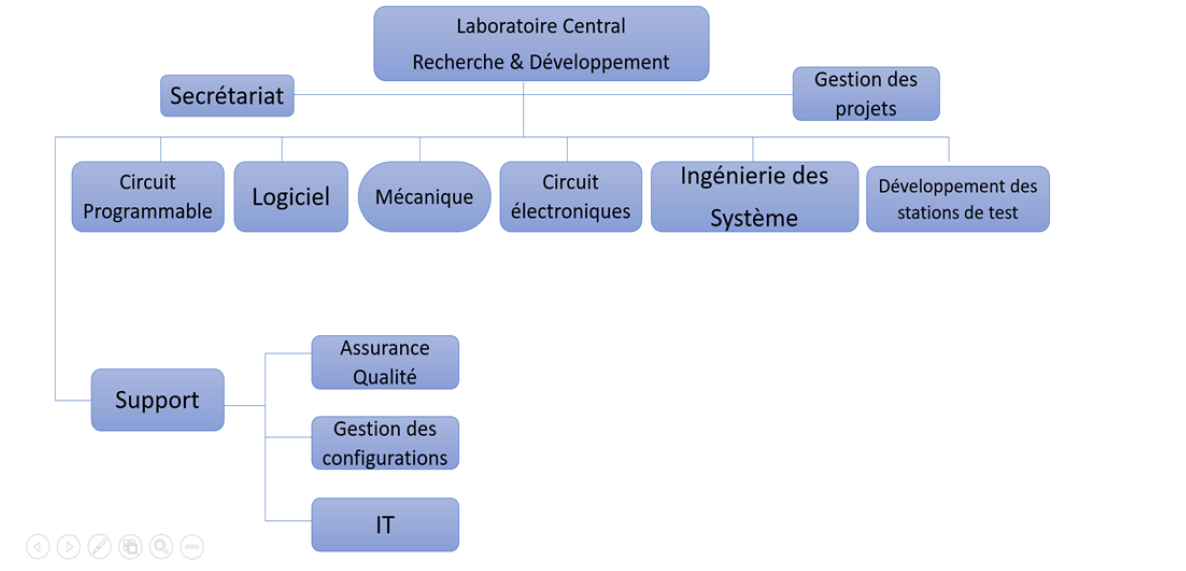
\includegraphics[width=0.9\textwidth]{./images/organigramme_rd.png}
    \caption{Organigramme fonctionnel du Laboratoire Central R\&D}
    \label{fig:organigramme_rd}
\end{figure}

\subsection{Missions et activités du Laboratoire Central R\&D}
\label{subsec:missions_labo}

Le Laboratoire Central R\&D a pour mission principale le développement, l'innovation et l'intégration de solutions technologiques avancées dans le domaine des systèmes de transmissions.

\paragraph{Activités techniques}
\begin{itemize}
    \item Développement de solutions innovantes pour les systèmes de transmissions de nouvelle génération ;
    \item Recherche et développement de solutions logicielles pour systèmes embarqués ;
    \item Modélisation et implémentation sur circuits programmables ;
    \item Conception électronique : choix d'architecture, schématisation, routage PCB ;
    \item Conception mécanique des produits et choix des matériaux ;
    \item Simulation des modèles (thermique, mécanique, etc.) ;
    \item Développement des processus et bancs de test ;
    \item Conception des interfaces de test.
\end{itemize}

\paragraph{Tâches managériales}
\begin{itemize}
    \item Gestion et planification des ressources de développement ;
    \item Analyse des risques et opportunités ;
\end{itemize}

\subsection{Infrastructure du Laboratoire Central R\&D}
\label{subsec:infra_labo}

Le Laboratoire Central R\&D s’étend sur 672 m² (48 m $\times$ 14 m) et comprend :
\begin{itemize}
    \item Quatorze (14) bureaux pour développeurs (répartis par spécialité) ;
    \item Bureau du gestionnaire des projets ;
    \item Bureau du chef de laboratoire ;
    \item Deux (02) centres de test (Hardware et Software) ;
    \item Deux (02) magasins (Hardware et Software) ;
    \item Salle de réunion ;
    \item Salle des machines ;
    \item Salle des serveurs ;
    \item Magasin pour matériel informatique ;
    \item Réception.
\end{itemize}

\subsection{Objectifs à long terme}
\label{subsec:objectifs_labo}

\begin{itemize}
    \item Augmenter le taux d’intégration dans la fabrication des équipements de transmissions ;
    \item Développer des compétences pour la conception de nouveaux équipements ;
    \item Renforcer les capacités en gestion de projets R\&D ;
    \item Concevoir des solutions adaptées aux besoins opérationnels, conformes aux normes internationales.
\end{itemize}


\end{document}

%==================== CHAPITRE 2 ====================
\chapter{Contexte et problématique}

\section{Contexte technologique}

L’industrie moderne exige des systèmes intelligents capables d’anticiper les pannes et de protéger les réseaux industriels.

\section{Problématique}

Comment concevoir un système capable de :

\begin{itemize}
\item Détecter les défauts mécaniques.
\item Prédire les défaillances.
\item Sécuriser les communications IIoT.
\end{itemize}

%==================== CHAPITRE 3 ====================
\chapter{Conception et Réalisation du Système}

\section{Architecture générale}

Le système repose sur :

\begin{itemize}
\item Capteurs intelligents
\item ROS2
\item Modèle IA CNN-LSTM
\item Secure Gateway
\item Tableau de bord de supervision
\end{itemize}

\section{Modules logiciels}

Chaque composant communique via ROS2 avec échange de données temps réel.

%==================== CHAPITRE 4 ====================
\chapter{Validation Expérimentale}

\section{Scénarios de test}

Plusieurs scénarios ont été simulés :

\begin{itemize}
\item Fonctionnement normal
\item Défaut roulement
\item Surchauffe
\item Déséquilibre
\item Attaque DDoS
\end{itemize}

\section{Résultats}

Le système a montré une bonne précision de détection avec une faible latence.

%==================== CONCLUSION ====================
\chapter*{Conclusion Générale}
\addcontentsline{toc}{chapter}{Conclusion Générale}

Ce travail a permis de développer un prototype intelligent combinant maintenance prédictive et cybersécurité industrielle.

Les résultats obtenus démontrent l’intérêt des jumeaux numériques dans les environnements industriels modernes.

%==================== BIBLIO ====================
\begin{thebibliography}{9}

\bibitem{ind4}
Industrie 4.0 et transformation numérique.

\bibitem{iot}
Applications de l’IIoT en maintenance prédictive.

\bibitem{ai}
Deep Learning for Predictive Maintenance.

\end{thebibliography}
\section{Le Circuit Intégré NE555}

\subsection{Introduction}

Le NE555 est un circuit intégré très populaire utilisé dans les montages électroniques. Il a été conçu en 1971 par \textit{Hans R. Camenzind} pour la société \textit{Signetics}. Grâce à sa simplicité, son faible coût et sa grande polyvalence, le NE555 est largement utilisé dans les domaines de l’électronique analogique et numérique.

Le NE555 peut fonctionner dans plusieurs modes :
\begin{itemize}
    \item Mode monostable
    \item Mode astable
    \item Mode bistable
\end{itemize}

Il est principalement utilisé pour :
\begin{itemize}
    \item La génération d’impulsions
    \item Les temporisations
    \item Les oscillateurs
    \item La modulation PWM
    \item Les clignoteurs LED
    \item Les alarmes et minuteries
\end{itemize}

\subsection{Structure Interne du NE555}

Le NE555 est composé de plusieurs blocs internes :
\begin{itemize}
    \item Deux comparateurs
    \item Une bascule RS (Flip-Flop)
    \item Un transistor de décharge
    \item Un pont diviseur constitué de trois résistances de 5k$\Omega$
\end{itemize}

Le pont diviseur crée deux tensions de référence :
\[
\frac{1}{3}V_{CC} \quad \text{et} \quad \frac{2}{3}V_{CC}
\]

Ces tensions sont utilisées par les comparateurs pour contrôler l’état de sortie du circuit.

\subsection{Brochage du NE555}

Le NE555 possède 8 broches :

\begin{table}[H]
\centering
\begin{tabular}{|c|c|p{8cm}|}
\hline
\textbf{Broche} & \textbf{Nom} & \textbf{Fonction} \\
\hline
1 & GND & Masse du circuit \\
\hline
2 & Trigger & Déclenchement du temporisateur \\
\hline
3 & Output & Sortie du signal \\
\hline
4 & Reset & Réinitialisation du circuit \\
\hline
5 & Control Voltage & Contrôle de la tension de référence \\
\hline
6 & Threshold & Comparaison du seuil de tension \\
\hline
7 & Discharge & Décharge du condensateur \\
\hline
8 & VCC & Alimentation du circuit \\
\hline
\end{tabular}
\caption{Description des broches du NE555}
\end{table}

\subsection{Caractéristiques Techniques}

\begin{itemize}
    \item Tension d’alimentation : 4.5V à 16V
    \item Courant de sortie maximal : environ 200 mA
    \item Fréquence de fonctionnement : jusqu’à plusieurs centaines de kHz
    \item Faible coût et haute fiabilité
    \item Compatible avec les circuits TTL et CMOS
\end{itemize}

\subsection{Mode Monostable}

Dans le mode monostable, le NE555 produit une seule impulsion lorsqu’il reçoit un signal de déclenchement.

La durée de l’impulsion dépend de la résistance \(R\) et du condensateur \(C\) :

\[
T = 1.1 \times R \times C
\]

où :
\begin{itemize}
    \item \(T\) : durée de l’impulsion (s)
    \item \(R\) : résistance ($\Omega$)
    \item \(C\) : capacité (F)
\end{itemize}

\subsubsection{Applications du mode monostable}

\begin{itemize}
    \item Temporisateur
    \item Détection d’impulsion
    \item Commande automatique
\end{itemize}

\subsection{Mode Astable}

Dans le mode astable, le NE555 fonctionne comme un oscillateur et produit un signal carré continu.

La fréquence du signal est donnée par :

\[
f = \frac{1.44}{(R_1 + 2R_2)C}
\]

Le temps à l’état haut :

\[
T_H = 0.693(R_1 + R_2)C
\]

Le temps à l’état bas :

\[
T_B = 0.693(R_2)C
\]

La période totale :

\[
T = T_H + T_B
\]

\subsubsection{Applications du mode astable}

\begin{itemize}
    \item Générateur d’horloge
    \item Clignotement de LED
    \item Génération de signaux PWM
    \item Oscillateur audio
\end{itemize}

\subsection{Mode Bistable}

En mode bistable, le NE555 agit comme une mémoire possédant deux états stables :
\begin{itemize}
    \item Etat haut
    \item Etat bas
\end{itemize}

Le changement d’état dépend des signaux appliqués sur les entrées \textit{Trigger} et \textit{Reset}.

\subsection{Avantages du NE555}

\begin{itemize}
    \item Simplicité d’utilisation
    \item Faible coût
    \item Grande stabilité
    \item Large plage d’alimentation
    \item Polyvalence
\end{itemize}

\subsection{Inconvénients du NE555}

\begin{itemize}
    \item Consommation relativement élevée
    \item Précision limitée pour les temporisations longues
    \item Sensibilité aux parasites dans certains montages
\end{itemize}

\subsection{Applications Pratiques}

Le NE555 est utilisé dans plusieurs domaines :
\begin{itemize}
    \item Electronique industrielle
    \item Robotique
    \item Systèmes embarqués
    \item Alarmes électroniques
    \item Variateurs de vitesse
    \item Générateurs de fréquence
\end{itemize}

\subsection{Conclusion}

Le circuit intégré NE555 est un composant essentiel dans le domaine de l’électronique grâce à sa simplicité et sa flexibilité. Il permet de réaliser facilement des fonctions de temporisation, d’oscillation et de génération d’impulsions. Malgré l’existence de microcontrôleurs modernes, le NE555 reste très utilisé dans les systèmes électroniques pour les applications simples et économiques.
\end{document}
\section{Le circuit intégré NE555}

Le \textbf{NE555} est un circuit intégré très utilisé en électronique pour générer des temporisations, des impulsions et des signaux carrés. Il a été conçu en 1971 par \textbf{Hans R. Camenzind} pour la société \textbf{Signetics}.

\subsection{Caractéristiques principales}

\begin{itemize}
    \item Tension d'alimentation : de 4,5 V à 16 V
    \item Faible coût et grande disponibilité
    \item Facile à utiliser
    \item Peut fonctionner en mode analogique ou numérique
    \item Courant de sortie jusqu'à 200 mA (selon version)
\end{itemize}

\subsection{Brochage du NE555}

Le NE555 possède \textbf{8 broches} :

\begin{enumerate}
    \item GND : masse
    \item Trigger : déclenchement
    \item Output : sortie
    \item Reset : remise à zéro
    \item Control Voltage : tension de contrôle
    \item Threshold : seuil
    \item Discharge : décharge
    \item VCC : alimentation positive
\end{enumerate}

\subsection{Modes de fonctionnement}

\subsubsection{Mode monostable}

Dans ce mode, le NE555 produit une seule impulsion lorsqu'il reçoit un signal de déclenchement.

Durée de l'impulsion :

\[
T = 1.1 \times R \times C
\]

où :

\begin{itemize}
    \item $T$ : temps en secondes
    \item $R$ : résistance en ohms
    \item $C$ : condensateur en farads
\end{itemize}

\subsubsection{Mode astable}

Dans ce mode, le NE555 génère un signal carré continu.

Fréquence :

\[
f = \frac{1.44}{(R_1 + 2R_2)C}
\]

Rapport cyclique :

\[
D = \frac{R_1 + R_2}{R_1 + 2R_2}
\]

\subsection{Applications}

\begin{itemize}
    \item Générateur d'horloge
    \item Clignotement de LED
    \item Temporisateur
    \item PWM
    \item Alarmes sonores
    \item Générateur d'impulsions
\end{itemize}

\subsection{Avantages}

\begin{itemize}
    \item Simple à utiliser
    \item Robuste
    \item Peu coûteux
    \item Très polyvalent
\end{itemize}

\subsection{Conclusion}

Le NE555 reste l'un des circuits intégrés les plus célèbres en électronique grâce à sa simplicité, sa fiabilité et ses nombreuses applications.